\documentclass[12pt, a4paper]{article}
\usepackage[english]{babel}
\usepackage{titlesec}

% \titleformat{\chapter} % command [display] % shape {\bfseries\huge} % format
%   {Chapter \thechapter} % label {0pt} % sep {} % before-code


\usepackage[T5]{fontenc}
\usepackage{mathptmx}[ptm]
\usepackage{a4wide, amssymb, epsfig, latexsym, array, hhline, fancyhdr}
\usepackage[normalem]{ulem}
%\usepackage{soul}
\usepackage{float}
\usepackage[makeroom]{cancel}
\usepackage{amsmath}
\usepackage{amsthm}
\usepackage{multicol, longtable, amscd}
\usepackage{diagbox}%Make diagonal lines in tables
\usepackage{booktabs}
\usepackage{alltt}
\usepackage[framemethod=tikz]{mdframed}% For highlighting paragraph backgrounds
\usepackage{indentfirst}
\usepackage{caption,subcaption}
\usepackage{svg}
\graphicspath{ {figures/} }
\usepackage{lastpage}
\usepackage[lined,boxed,commentsnumbered]{algorithm2e}
\usepackage{enumerate}
\usepackage{color}
\usepackage{graphicx}% Standard graphics package
\graphicspath{ {figures/} }
\usepackage{array}
\usepackage{tabularx, caption}
\usepackage{tabularray}
\usepackage{multirow}
\usepackage{multicol}
\usepackage{rotating}
\usepackage{graphics}
\usepackage{geometry}
\usepackage{setspace}
\usepackage{epsfig}
\usepackage{tikz}
\usepackage[numbers]{natbib}
\usepackage{subcaption}

\usepackage{dirtree}



\usetikzlibrary{arrows, snakes, backgrounds, calc}
\usepackage[unicode]{hyperref}
\hypersetup{urlcolor=blue,linkcolor=black,citecolor=black,colorlinks=true} 

\usepackage{xcolor}

\definecolor{codegreen}{rgb}{0,0.6,0}
\definecolor{codegray}{rgb}{0.5,0.5,0.5}
\definecolor{codepurple}{rgb}{0.58,0,0.82}
\definecolor{backcolour}{rgb}{0.95,0.95,0.92}

\usepackage{listings}
\lstdefinestyle{mystyle}{ backgroundcolor=\color{backcolour},   
    commentstyle=\color{codegreen}, keywordstyle=\color{magenta},
    numberstyle=\tiny\color{codegray}, stringstyle=\color{codepurple},
    basicstyle=\ttfamily\footnotesize, breakatwhitespace=false,         
    breaklines=true,                 
    captionpos=b,                    
    keepspaces=true,                 
    numbers=left,                    
    numbersep=5pt,                  
    showspaces=false,                
    showstringspaces=false, showtabs=false,                  
    tabsize=2 }
\lstset{style=mystyle}



\def\thesislayout{	% A4: 210 × 297
	\geometry{ a4paper, total={160mm,240mm},  % fix over page
		left=30mm, top=30mm, } }
\thesislayout

%\usepackage{fancyhdr}
\setlength{\headheight}{40pt}
\pagestyle{fancy}
\fancyhead{} % clear all header fields
\fancyhead[L]{
 \begin{tabular}{rl}
    \begin{picture}(25,15)(0,0) \put(0,-8){
\includegraphics[width=10mm,
    height=10mm]{Images/hcmut.png}}
    %\put(0,-8){\epsfig{width=10mm,figure=hcmut.eps}}
   \end{picture}&
	%
\includegraphics[width=8mm, height=8mm]{hcmut.png} & %
	\begin{tabular}{l}
        \textbf{ Ho Chi Minh City University of Technology } \\
        \textbf{ Faculty of Computer Science and Engineering }
	\end{tabular} 	
 \end{tabular}
} \fancyhead[R]{
	\begin{tabular}{l}
		\tiny \bf \\
		\tiny \bf \end{tabular}  } \fancyfoot{} % clear all footer fields
\fancyfoot[L]{\scriptsize Big data (CO5153) - Academic year 2024 - 2025}
\fancyfoot[R]{\scriptsize  Page {\thepage}/\pageref{LastPage}}
\renewcommand{\headrulewidth}{0.3pt}
\renewcommand{\footrulewidth}{0.3pt}

%%%%%%%%%%%%%%%%%%%%%%%%%%%%%%%%%%%%%%%%%%
% Tạo một môi trường mới cho các bảng đặc tả UC, giúp định dạng kiểu
\newenvironment{usecase_table}[1][Test]
{
\begin{table}[H]
% Left-Right Table padding
    \setlength{\tabcolsep}{6pt}
    \renewcommand{\arraystretch}{1.5}
    % \begin{tabularx}{\textwidth}{bs}
    \def\savedcaption{\caption{#1}}%
    \begin{tabular}{|>{\bfseries} p{0.2\linewidth}|p{0.7\linewidth}|}

} {
    \end{tabular}
    \savedcaption
\end{table}
}

\newenvironment{usecase_enum}
{
    \begin{enumerate*}[itemjoin={\newline}]
} {
    \end{enumerate*}
}

\makeatletter
\newenvironment{acknowledgments}{
	\small
	\begin{center}
	  {\bfseries Acknowledgments\vspace{-.5em}\vspace{\z@}}
	\end{center}
	\quotation
  }{}
\makeatother

% Declaration
\makeatletter
\newenvironment{declaration}{
	\small
	\begin{center}
	  {\bfseries Declaration\vspace{-.5em}\vspace{\z@}}
	\end{center}
	\quotation
  }{}
\makeatother

\makeatletter
\newenvironment{abstr}{
        \small
        \begin{center}
	{\bfseries Abstract \vspace{-.5em}\vspace{\z@}}
        \end{center}
        \quotation
    }{}
\makeatother

\makeatletter
\newenvironment{abstrsss}{
        \small
        \begin{center}
	{\bfseries Abstractss \vspace{-.5em}\vspace{\z@}}
        \end{center}
        \quotation
    }{}
\makeatother
%%%%%%%%%%%%%%%%%%%%%%%%%%%%%%%%%%%%%%%%%%%%%%5
\setcounter{secnumdepth}{4}
\setcounter{tocdepth}{3}
\makeatletter
\newcounter {subsubsubsection}[subsubsection]
\renewcommand\thesubsubsubsection{\thesubsubsection .\@alph\c@subsubsubsection}
\newcommand\subsubsubsection{\@startsection{subsubsubsection}{4}{\z@}%
                                     {-3.25ex\@plus -1ex \@minus -.2ex}%
                                     {1.5ex \@plus .2ex}%
                                     {\normalfont\normalsize\bfseries}}
\newcommand*\l@subsubsubsection{\@dottedtocline{3}{10.0em}{4.1em}}
\newcommand*{\subsubsubsectionmark}[1]{}
\makeatother



\everymath{\color{black}}%make in-line maths symbols blue to read/check easily

\sloppy
\captionsetup[figure]{labelfont={small,bf},textfont={small,it},belowskip=-1pt,aboveskip=-9pt}
%space removed between caption, figure, and text
\captionsetup[table]{labelfont={small,bf},textfont={small,it},belowskip=-1pt,aboveskip=7pt}
\setlength{\floatsep}{5pt plus 2pt minus 2pt}
\setlength{\textfloatsep}{5pt plus 2pt minus 2pt}
\setlength{\intextsep}{10pt plus 2pt minus 2pt}


% Declare a variable named Proc using \newcommand

\newcommand{\Uni}{Ho Chi Minh University - Vietnam National Unversity, Ho Chi Minh City}

\renewcommand{\labelitemi}{\normalfont\bfseries\textendash}
\renewcommand{\labelitemii}{\textbullet}
\renewcommand*\baselinestretch{1.5}\selectfont


\thesislayout

\begin{document}

\begin{titlepage}
    
\begin{tikzpicture}[remember picture, overlay]
        \draw[line width = 4pt] ($(current page.north west) + (1.0in,-0.5in)$)
        rectangle ($(current page.south east) + (-0.4in,0.5in)$);
        \draw[line width=1.5pt]
        ($ (current page.north west) + (1.05in,-0.55in) $) rectangle ($ (current
        page.south east) + (-0.45in,0.55in) $);
    \end{tikzpicture}

    \begin{center}
        \large \textbf{VIETNAM NATIONAL UNIVERSITY, HO CHI MINH CITY} \\
        \large \textbf{HO CHI MINH UNIVERSITY OF TECHNOLOGY} \\
        \large \textbf{FACULTY OF COMPUTER SCIENCE AND ENGINEERING}
    \end{center}

    \begin{figure}[h!]
        \begin{center}
            
\includegraphics[width=5cm]{Images/hcmut.png}
        \end{center}
    \end{figure}

    \begin{center}
        \begin{tabular}{c}
        \multicolumn{1}{l}{\textbf{{\Large Big Data (CO5153)}}}\\
        ~~\\
        \hline
        \\
        \multicolumn{1}{l}{\textbf{{\Large Assignment Report}}}\\
        \\
        \textbf{{\Huge Applying Streaming SQL in}}\\
        \textbf{{\Huge Real-Time Social Media}}\\
        \textbf{{\Huge Interaction Tracking}}\\
        \\
        \hline
        \end{tabular}
        \end{center}

    \vspace{1cm}
    \begin{table}[H]
        \begin{tabular}{rrl}
        \hspace{5 cm} & \textbf{Mentor}: & Thoại Nam \\
        
        & \textbf{Student}: & Trần Hà Tuấn Kiệt -- 2011493 \\
        & & Nguyễn Đức Thuỵ -- 2012158 \\
        \end{tabular}
        \end{table}
    \vspace{1cm}

    \begin{center}
        {\large Ho Chi Minh City, \the\month/\the\year}
    \end{center}
\end{titlepage}


\newpage

%\thispagestyle{empty} \chapter*{Work Assignment} \begin{table}[H] \centering
% \renewcommand{\arraystretch}{1.5} \begin{tabular}{|c|c|c|l|} \hline
% \textbf{No.}       & \textbf{Full name}                 & \textbf{Student ID}
% & \textbf{Work Assignment}                     \\
%         \hline %%%%%Student 1%%%%%%%%%%% \multirow{4}{*}{1} &
%         \multirow{4}{*}{Trần Hà Tuấn Kiệt} & \multirow{4}{*}{2011493} & -
%         Exploratory Data Analysis                  \\
%                            &                                    &
%                            & - System proposal and architecture           \\
%                            &                                    &
%                            & - Research and Develop with new technologies \\
%                            &                                    &
%                            & - Implement system endpoints                 \\
%         \hline %%%%%Student 2%%%%%%%%%%% \multirow{4}{*}{2} &
%         \multirow{4}{*}{Nguyễn Đức Thuỵ}   & \multirow{4}{*}{2012158} & -
%         Exploratory Data Analysis                  \\
%                            &                                    &
%                            & - System proposal and architecture           \\
%                            &                                    &
%                            & - Research and Develop with new technologies \\
%                            &                                    &
%                            & - Implement data processing flows            \\
%         \hline \end{tabular} \end{table} \newpage

% Revert title name back to English
\renewcommand{\contentsname}{Table of Contents}
\renewcommand{\listfigurename}{List of Figures}
\renewcommand{\listtablename}{List of Tables}
\renewcommand{\bibname}{References}
\renewcommand{\figurename}{Figure}

\tableofcontents
\newpage

%\thispagestyle{empty}
\listoffigures
\listoftables
\newpage

% \renewcommand\thechapter{Chapter \arabic{chapter}}

\section{Introduction about Social media Interaction}
\textbf{Social Media Interaction} refers to the ways users engage and
communicate with content, brands, and other users on social media platforms. It
encompasses all forms of engagement, such as likes, comments, shares, mentions,
direct messages, and reactions to posts. These interactions create a dynamic,
two-way communication channel between individuals, communities, and businesses.

Social media interaction encompasses various elements that enable engagement and
communication among users, brands, and communities. Engagement types like likes,
comments, shares, retweets, and mentions, which allow users to express opinions
and amplify content. Direct communication, such as private messages and replies,
facilitates personal connections, while user-generated content (UGC) like
reviews and testimonials highlights the creative involvement of users.
Additionally, community engagement through group discussions and forums fosters
a sense of belonging and collaboration. 

The importance of social media interaction lies in its ability to provide
real-time feedback, offering valuable insights into audience opinions,
preferences, and sentiments. It enhances brand awareness by increasing
visibility and trust, while also allowing businesses to analyze content
performance and measure campaign success. Social media interaction builds strong
relationships between brands and their audiences, encourages loyalty, and helps
identify emerging trends and consumer behaviors. Ultimately, it serves as a
powerful tool for driving meaningful connections and strategic growth in the
digital landscape.

This concept underscores the importance of leveraging unbounded data streams to
stay competitive in the dynamic world of digital engagement. The accompanying
vibrant image of individuals in creative poses reflects the dynamic and lively
nature of social media platforms, aligning with the essence of constant
interaction and engagement.

Let's take a look at a comparison between bounded dataset and unbounded dataset
in data processing.

\begin{figure}[H]
    \centering
    \includegraphics[width=\textwidth]{Images/unbounded-data.png}
    \vspace{1em}
    \caption{Comparison between bounded dataset and unbounded dataset. Source: Arroyo}
    \label{fig:comparison}
\end{figure}

\textbf{A table represents a bounded dataset}, meaning it contains a finite and
complete set of data at any given time. This bounded nature allows for aggregate
or summary calculations, such as counting records or calculating averages. For
example, the query \textbf{`SELECT count(*) FROM orders WHERE price > 100`} can
aggregate the results in the table to produce a deterministic count because the
data is static and complete.

On the other hand, \textbf{streams represent unbounded dataset}, where data
continuously flows in overtime. Since streams are ongoing, queries on streams
never actually end; they continuously process incoming data. For example, when
applying the same query to a stream, each incoming event is processed
individually, providing incremental updates to the results. This behavior is
suitable for scenarios such as real-time analytics or monitoring, where data is
continuously generated and processed.

In short, the \textbf{Figure \ref{fig:comparison}} demonstrates this distinction
effectively, showing how tables aggregate finite data into a static result,
while streams generate dynamic, continuously updated outputs. This concept is
essential in understanding how modern data systems like databases, stream
processors, and big data frameworks handle and process information.

\section{Problem Statement}
    \subsection{Impact}
    \textbf{The lack of real-time insights from unbounded social data}
    significantly hampers the ability of businesses and organizations to respond
    promptly to trends and audience engagement. In the fast-paced digital
    landscape, trends evolve rapidly, and audience preferences shift
    dynamically. Without continuous access to real-time data streams, it becomes
    difficult to monitor and analyze social interactions effectively. This delay
    in gaining actionable insights prevents organizations from adapting
    strategies, capitalizing on emerging opportunities, or addressing potential
    challenges in a timely manner. Ultimately, the inability to respond to
    real-time engagement can lead to missed opportunities, reduced
    competitiveness, and weakened connections with audiences, making it crucial
    to leverage tools that process unbounded data streams for effective
    decision-making and sustained growth.
    \subsection{Objectives}
    The objective is to \textbf{implement a real-time social media interaction
    tracking system for platforms} like Mastodon and X (formerly Twitter). This
    system will process and analyze unbounded streams of social media data,
    enabling organizations to monitor user interactions, engagement trends, and
    audience behaviors as they happen. By providing actionable insights in real
    time, it empowers businesses to stay responsive to emerging trends, adapt
    strategies effectively, and maintain relevance in the fast-paced digital
    landscape. This highlights the importance of leveraging advanced data
    processing technologies to manage the dynamic nature of social media,
    ensuring informed and timely decision-making.

    \subsection{Approach}
        \subsubsection{Data Collection}
            \subsubsubsection*{Mastodon}
            Mastodon is a decentralized social media platform structured as a
            \textbf{network of independent servers}, commonly referred to as
            instances. Each instance operates independently, serving unique
            communities and interests, yet they remain interconnected through a
            federated network. This decentralized approach contrasts with
            centralized platforms, fostering diversity and community-specific
            experiences.
            \begin{itemize}
                \item \textbf{Structure:} Mastodon's ecosystem consists of
                multiple independent servers, each catering to distinct
                communities while participating in a larger, interconnected
                federation.
                \item \textbf{Data access:} Mastodon provides real-time data
                streams through its Server-Sent Events (SSE) API, enabling
                access to ongoing activities like posts, mentions, hashtags, and
                interactions.
                \item \textbf{Data types:} The platform generates various types
                of data, including posts, mentions, hashtags, and user
                interactions, making it a rich source for social media analytics
                and engagement monitoring.
            \end{itemize}
            $\quad$ Mastodon presents unique challenges due to its decentralized
            structure, where data is distributed across numerous independent
            servers (instances). Aggregating and analyzing data from the entire
            network is inherently complex and resource-intensive, requiring
            sophisticated solutions to handle the fragmented ecosystem.
            Additionally, Mastodon's strong emphasis on user privacy, with
            strict controls and regulations, further complicates data collection
            and processing while ensuring compliance with user preferences and
            privacy standards.
            \subsubsubsection*{X (formerly Twitter)}
            X, formerly known as Twitter, operates as a centralized social media
            platform with a unified database, making it distinct from
            decentralized systems like Mastodon. This centralized structure
            provides a single, cohesive source of data, which simplifies access
            and analysis for users, developers, and organizations.
            \begin{itemize}
                \item \textbf{Structure:} X is built on a centralized database
                architecture, enabling streamlined data management and easier
                access to platform-wide information.
                \item \textbf{Data access:} The platform offers real-time
                streams through the X API, allowing developers to track
                activities such as tweets, retweets, likes, mentions, and
                trending topics in real time.
                \item \textbf{Data types:} X generates various types of valuable
                data, including tweets, retweets, likes, mentions, and trends,
                making it a vital source for social media analytics and
                insights.
            \end{itemize}
            $\quad$ X faces notable challenges in its data access and usage policies.
            Strict \textbf{rate limits on API usage} restrict the volume of data that
            can be collected within a specific timeframe, creating barriers to
            conducting comprehensive and large-scale analyses. Additionally,
            \textbf{privacy regulations and API restrictions} further complicate data
            collection and processing, as developers and researchers must
            navigate limitations designed to protect user data while ensuring
            compliance with legal and ethical standards. These challenges
            necessitate innovative solutions to effectively leverage the
            platform's data while respecting its constraints.
            \subsubsection{Concept}
            \textbf{Streaming SQL} is an extension of traditional SQL, specifically designed to handle unbounded, real-time data streams. Unlike standard SQL, which processes finite datasets stored in static tables, Streaming SQL operates on continuous data streams that are constantly being updated, enabling real-time analysis and processing.
            \begin{figure}[H]
                \centering
                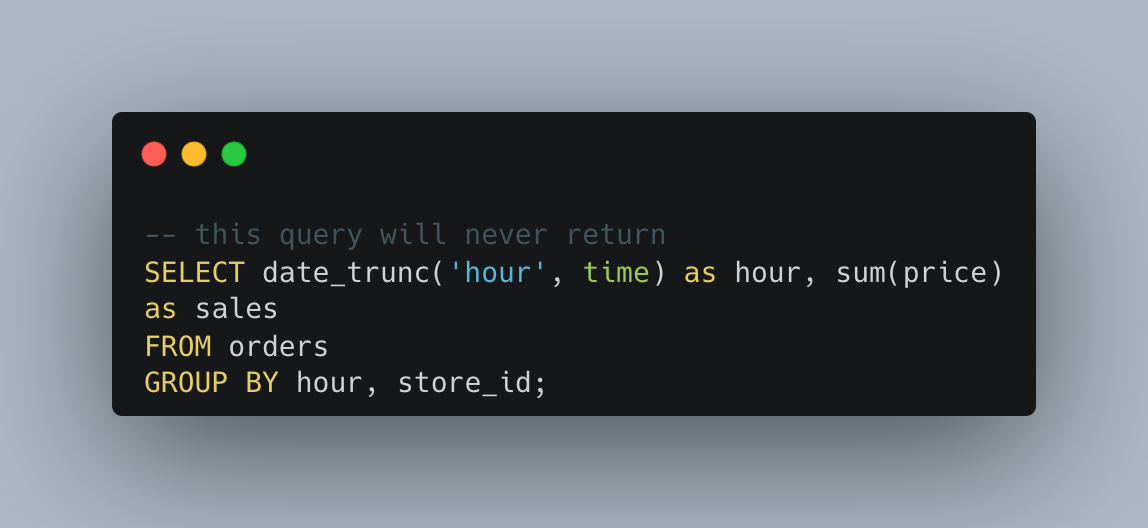
\includegraphics[width=0.7\textwidth]{Images/image (1).png}
                \vspace{1em}
                \caption{Concept of Streaming SQL}
            \end{figure}
            \begin{figure}[H]
                \centering
                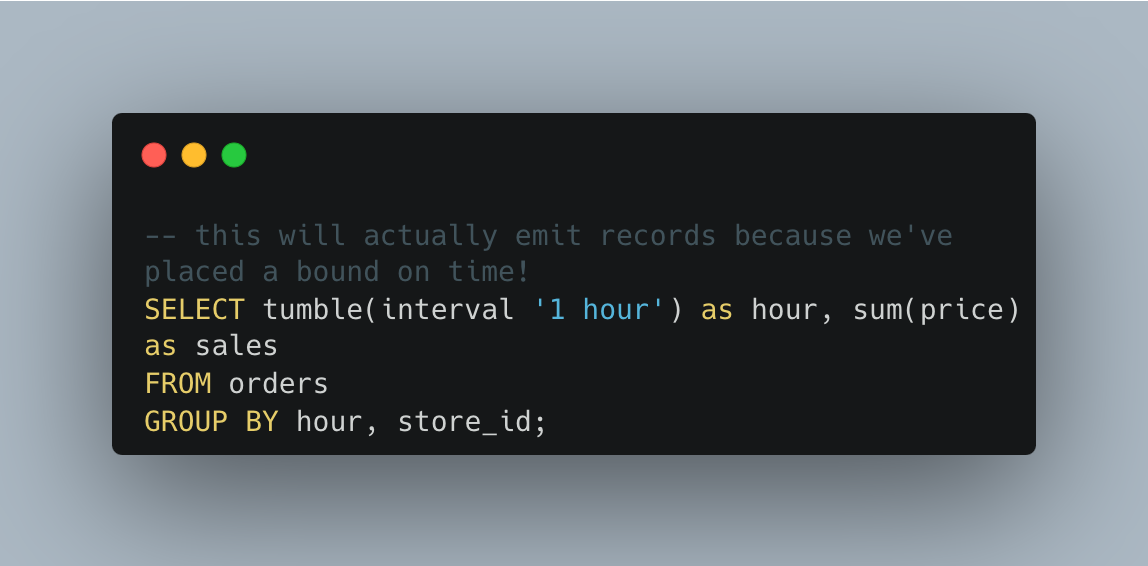
\includegraphics[width=0.7\textwidth]{Images/image (2).png}
                \vspace{1em}
                \caption{Concept of Streaming SQL}
            \end{figure}
            \subsubsubsection*{Dataflow Semantics}
            \begin{figure}[H]
                \centering
                
\includegraphics[width=0.7\textwidth]{Images/row-by-row.png}
                \vspace{1em}
                \caption{Row-by-Row Processing}
            \end{figure}
            \begin{figure}[H]
                \centering
                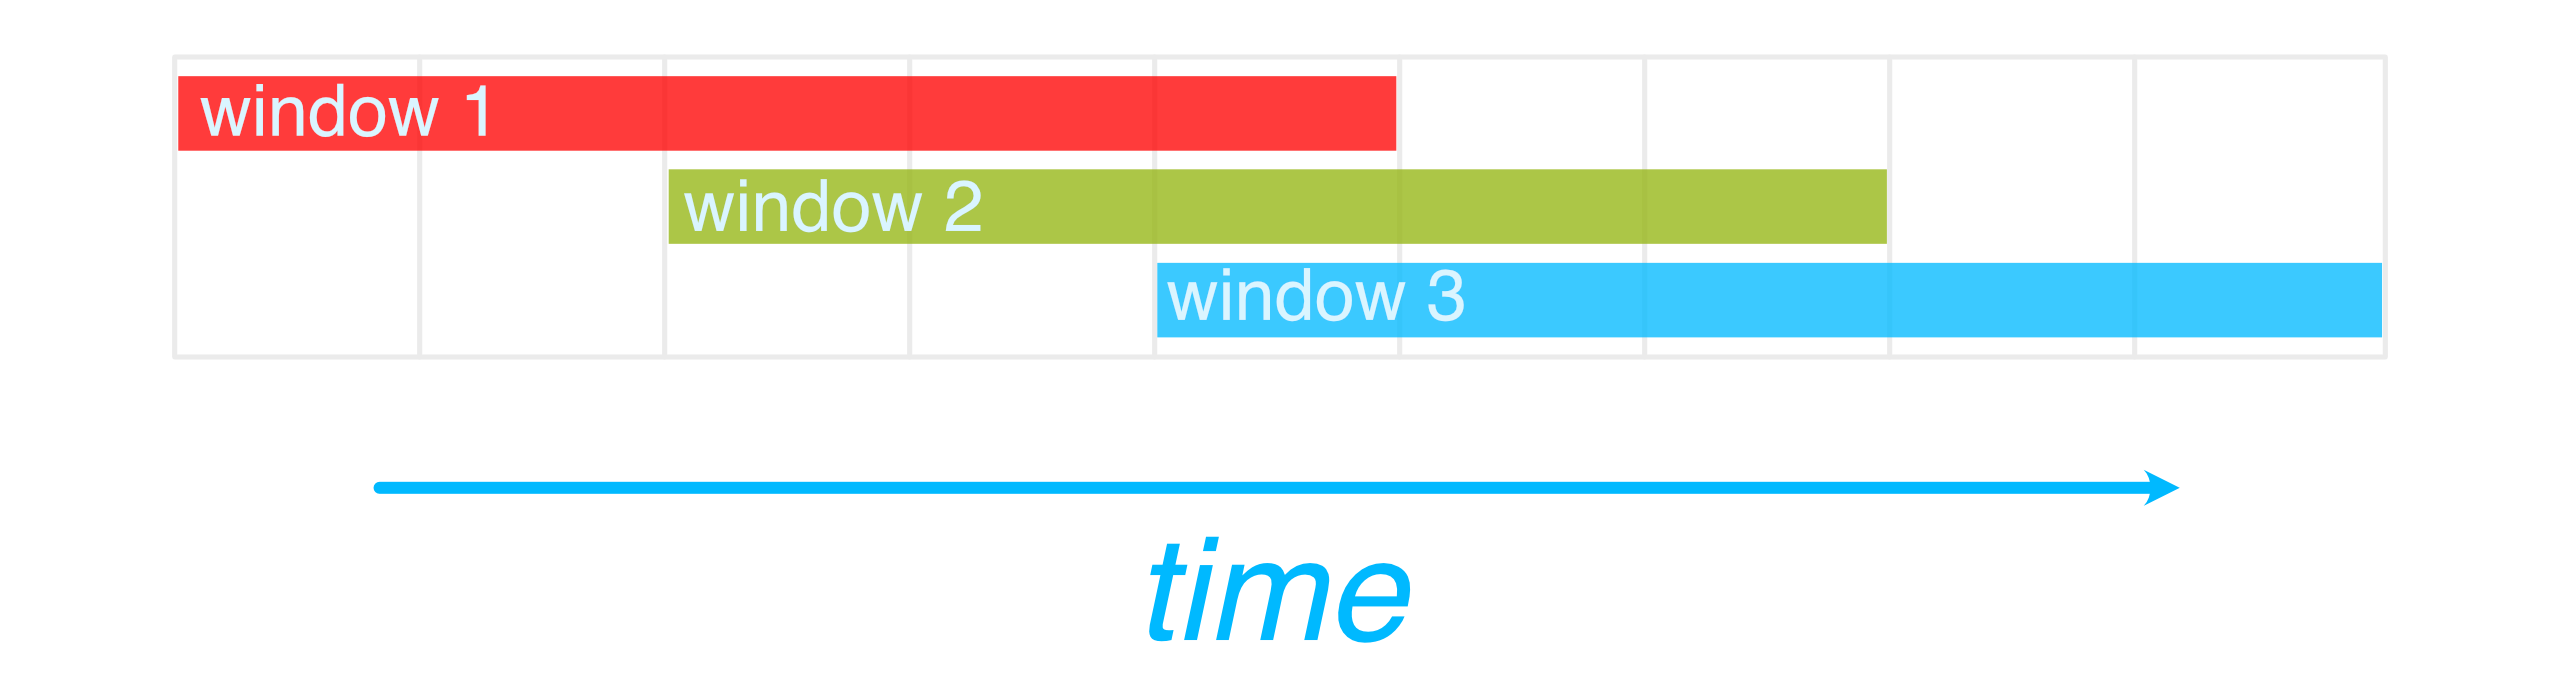
\includegraphics[width=0.7\textwidth]{Images/sliding-window.png}
                \vspace{1em}
                \caption{Sliding windows. Source: Arroyo}
            \end{figure}
            \begin{figure}[H]
                \centering
                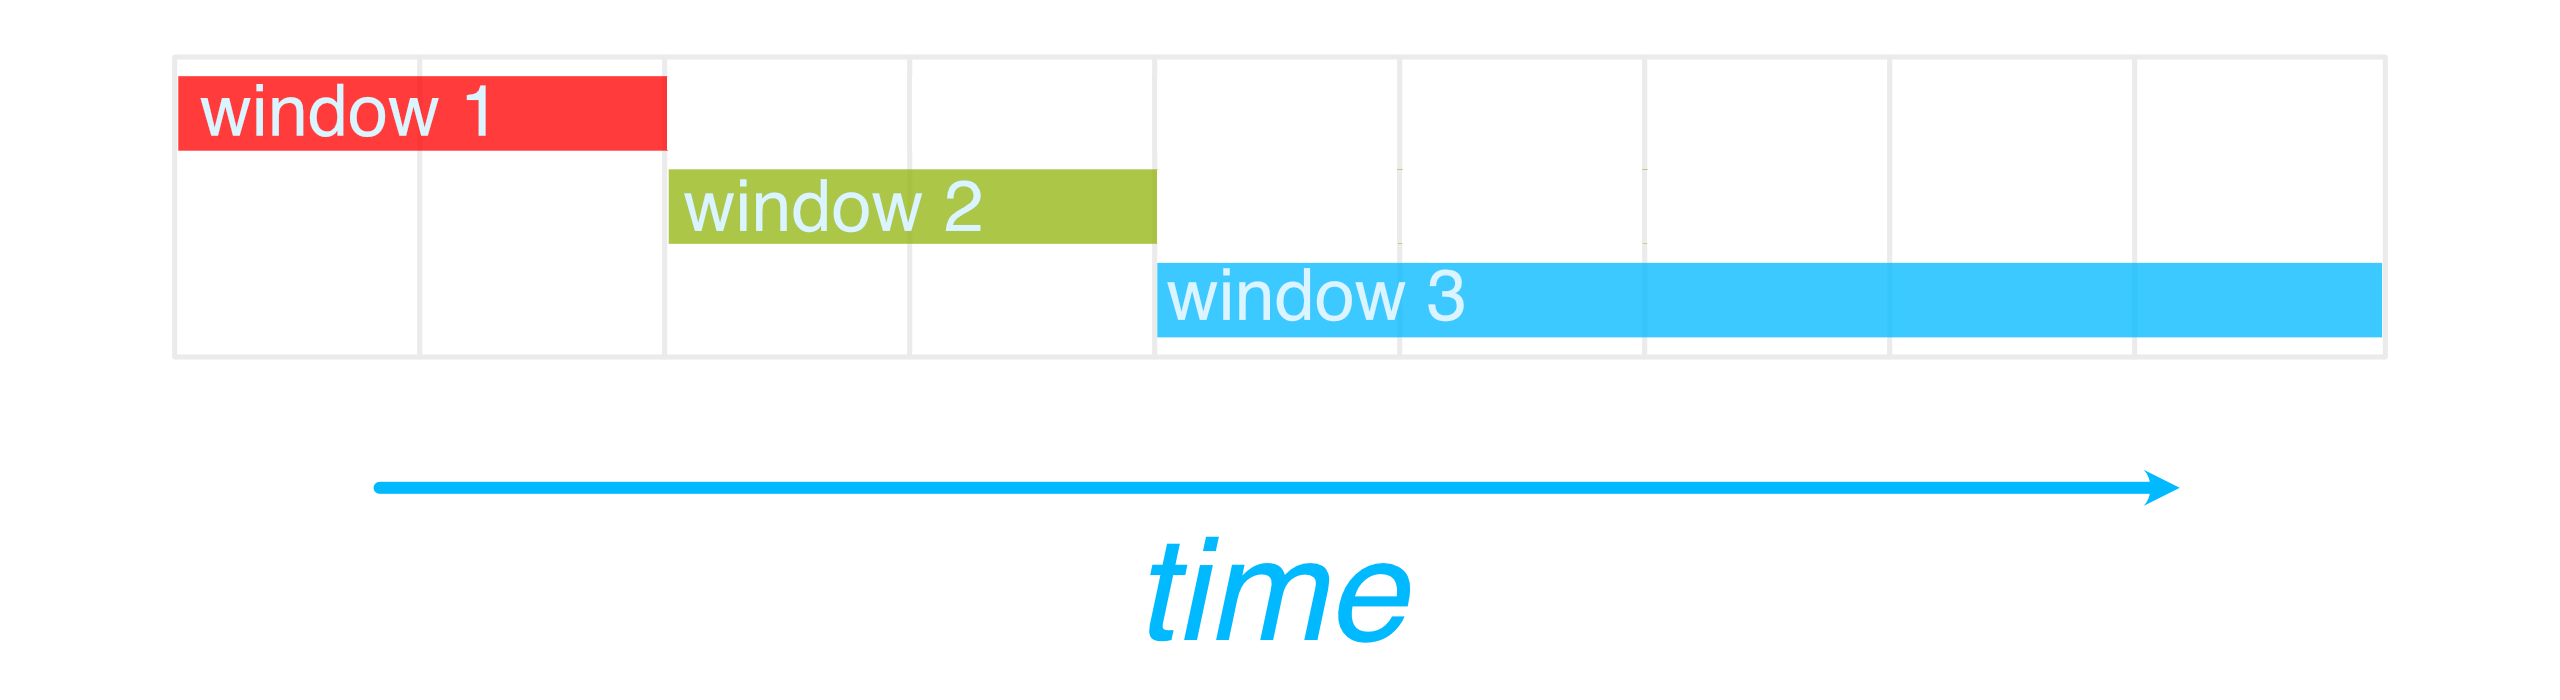
\includegraphics[width=0.7\textwidth]{Images/tumbling-window.png}
                \vspace{1em}
                \caption{Tumbling windows. Source: Arroyo}
            \end{figure}
            \begin{figure}[H]
                \centering
                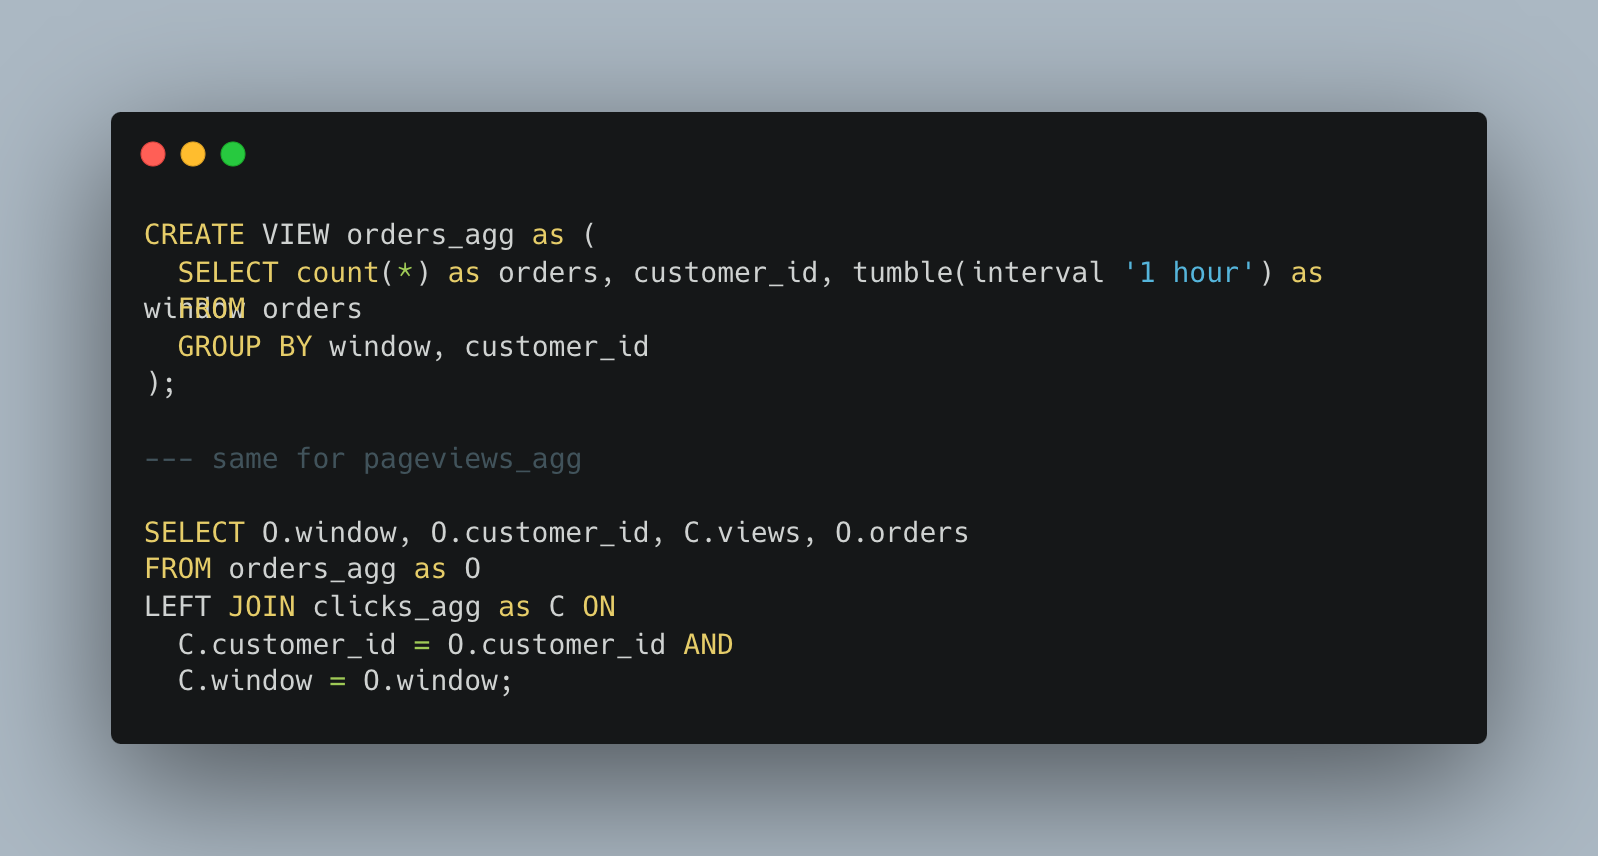
\includegraphics[width=0.7\textwidth]{Images/apply-JOIN.png}
                \vspace{1em}
                \caption{Apply to Join Operation}
            \end{figure}
            \subsubsubsection*{Update Semantics}
            \begin{figure}[H]
                \centering
                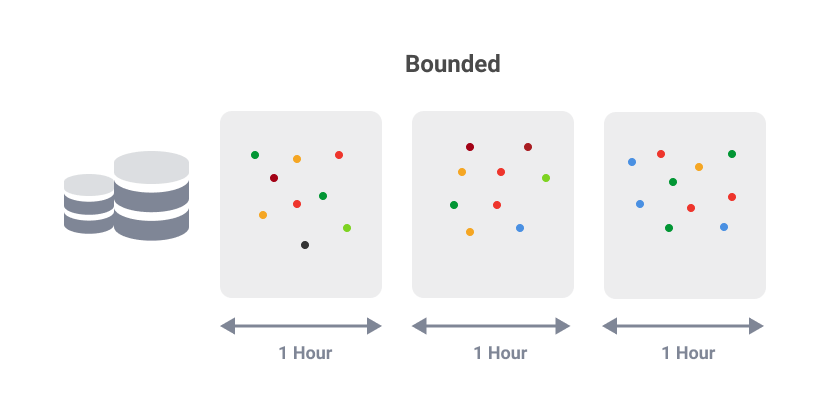
\includegraphics[width=0.7\textwidth]{Images/bounded-data-in-time.png}
                \vspace{1em}
                \caption{Bounded Data in Time}
            \end{figure}
            \begin{figure}[H]
                \centering
                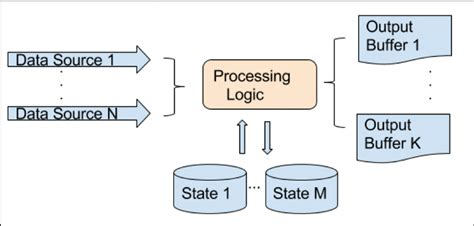
\includegraphics[width=0.7\textwidth]{Images/image (6).png}
                \vspace{1em}
                \caption{Processing logic of Incremental Updates}
            \end{figure}
        
        \subsubsection{Tool}
        \begin{figure}[H]
            \centering
            
\includegraphics[width=0.3\textwidth]{Images/arroyo.png}
            \vspace{1em}
            \caption{Arroyo}
        \end{figure}
        We will incorporate \textbf{Arroyo}, a distributed stream processing engine developed in Rust, as part of our technology stack to handle real-time data streams efficiently. Arroyo is designed to support SQL-based queries, making it accessible for processing large volumes of unbounded data streams with ease. Its high scalability ensures that it can handle significant workloads while maintaining \textbf{exactly-once semantics}, which is critical for ensuring data accuracy and consistency. This tool will enable us to implement robust, real-time data processing pipelines, making it an ideal choice for applications requiring low-latency and fault-tolerant stream analytics.
        \begin{figure}[H]
            \centering
            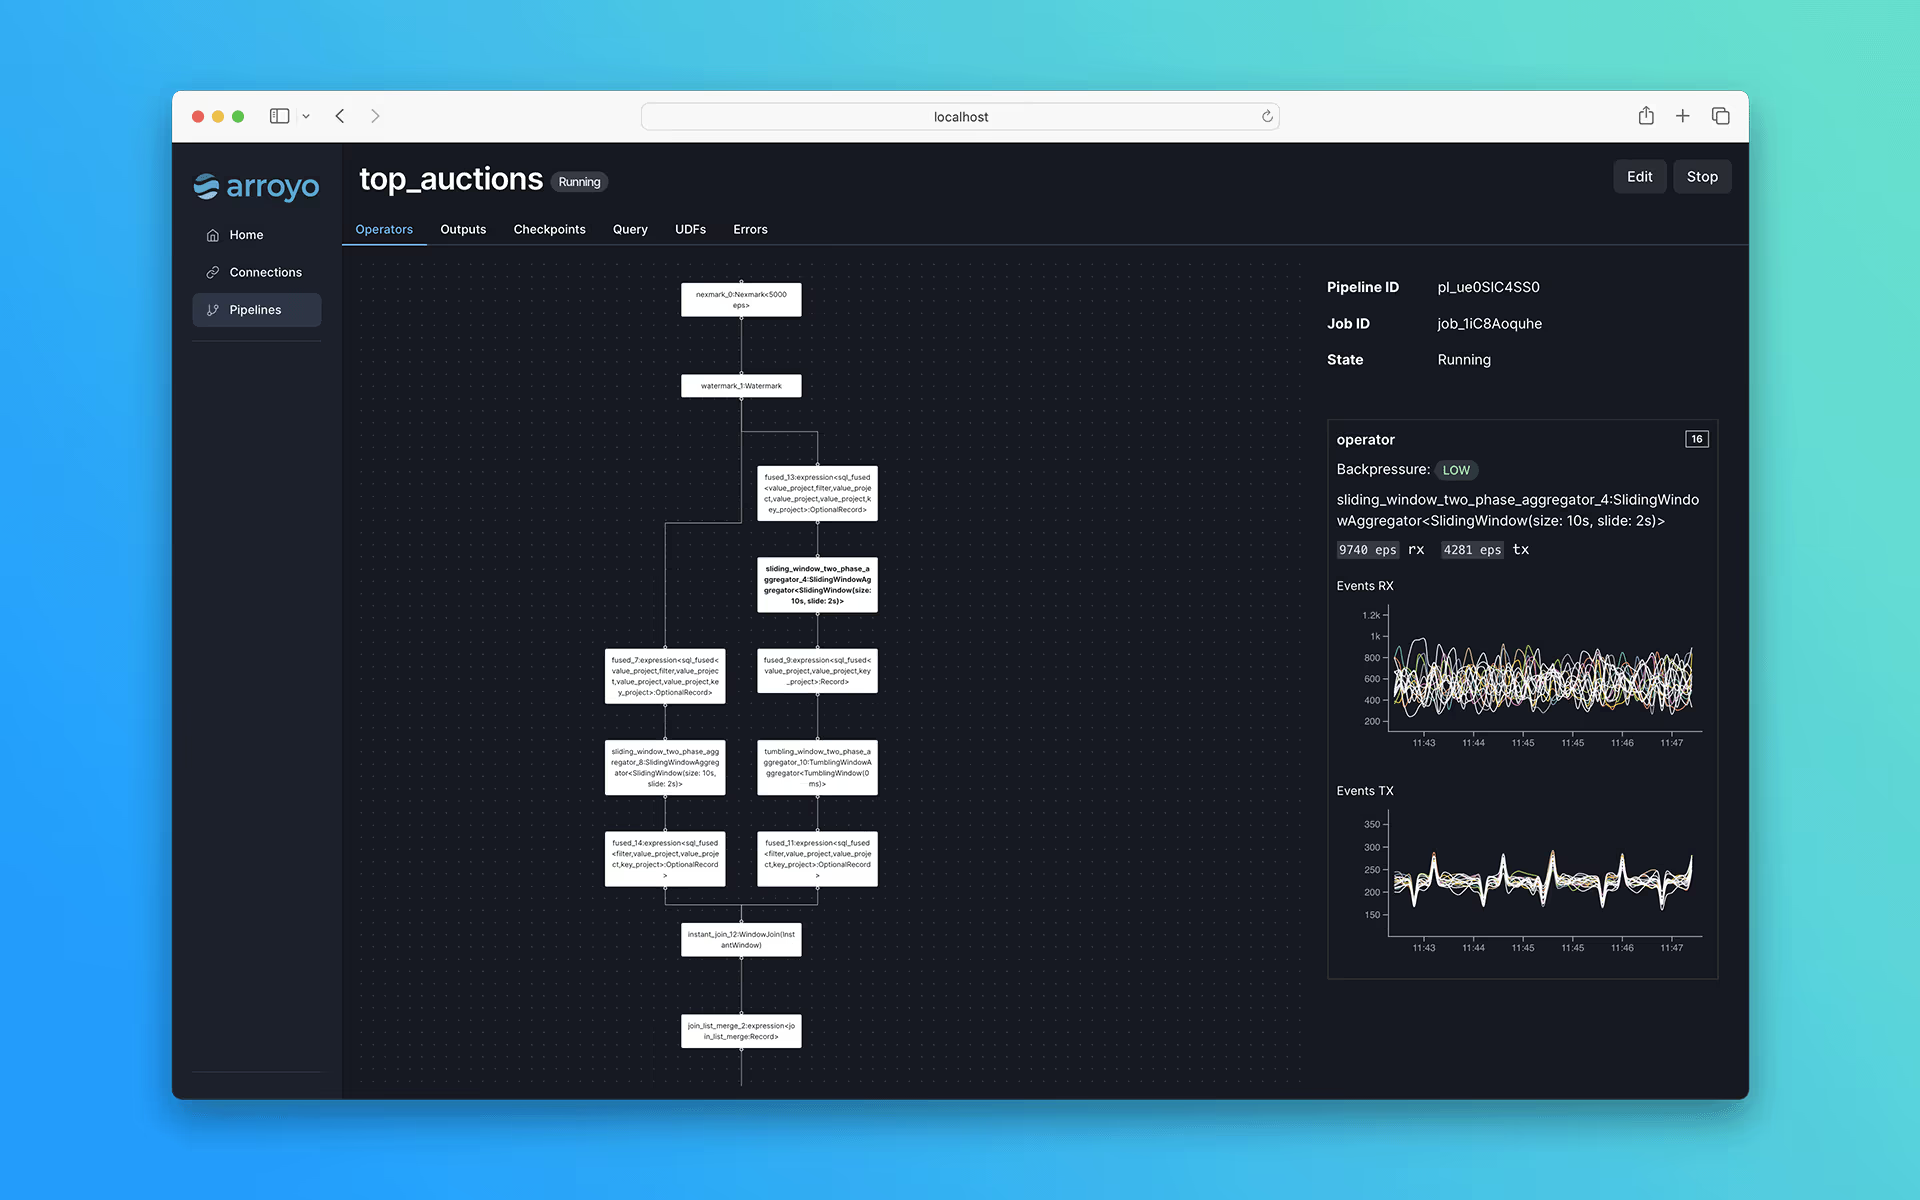
\includegraphics[width=\textwidth]{Images/tool-dash.png}
            \vspace{1em}
            \caption{Arroyo Dashboard. Source: Arroyo}
        \end{figure}

\section{Implementation}
In order to gain deeper insights into the operational dynamics and performance characteristics of
decentralized social media platforms, our team has undertaken an innovative demonstration project
leveraging the capabilities of Arroyo, a cutting-edge stream processing framework, to develop and
implement a sophisticated event processing system specifically designed to monitor and analyze
real-time activities across the Mastodon social network federation. This comprehensive monitoring
solution serves multiple strategic objectives, including the evaluation of user engagement patterns,
the assessment of network performance metrics, and the development of a more nuanced understanding
of how decentralized social media architectures function in practice. Through this implementation,
we aim to not only demonstrate the practical applications of stream processing technology in social
media analytics but also to contribute valuable insights to the growing body of knowledge
surrounding alternative social networking models that prioritize user privacy, data sovereignty, and
community-driven governance structures.

\subsection{Mastodon}
Mastodon represents a new approach to social networking through decentralized architecture. Rather
than operating as a single centralized platform controlled by one company, Mastodon functions as a
network of independently operated servers, known as instances. Each instance runs on open-source
software and communicates with other instances through a standardized protocol called ActivityPub
\cite{La_Cava_2021,w3c_2018}.

Mastodon has emerged as the most prominent platform within the Fediverse, offering functionality
comparable to traditional social media services. Users can share short-form content called "toots"
(similar to tweets) and amplify others' content through "boosts" (similar to retweets). The platform
also incorporates community-focused features reminiscent of Reddit, with independent communities
managed through separate instances, each with its own moderation policies.

The federated architecture of Mastodon serves as the foundation for our demonstration results,
utilizing a sophisticated event-driven approach to track and analyze instance activity across the
network. From a technical implementation perspective, the system operates by monitoring update
events across all participating Mastodon instances through a specialized Server-sent event
protocol \cite{html_standard_2024}, which broadcasts these events to a designated endpoint whenever a
user performs any update action within the network \cite{mastodon_ggmbh_2022}. Our technical
infrastructure systematically processes this event stream by first consuming the incoming events,
then performing data extraction to isolate the instance domain information from the event payload,
followed by implementing a rolling time-window aggregation mechanism that operates on 5-minute
intervals to calculate the frequency of updates originating from each domain instance. The
culmination of this processing pipeline results in the identification and selection of the five most
active instances, determined by their respective update frequencies, which provides valuable
insights into the distribution of user activity across the Mastodon federation network and helps us
understand the patterns of engagement within the decentralized social media landscape.

\subsection{Set Up Infrastructure}
For our experimental infrastructure implementation, we made a strategic decision to deploy Arroyo on
a Raspberry Pi model 3B+, a choice that aligns with our objectives to evaluate stream processing
capabilities on accessible hardware platforms. Our server configuration encompasses a 1.4GHz 64-bit
quad-core ARM Cortex-A53 processor complemented by 1 GB LPDDR2 SDRAM, with network connectivity
provided through Gigabit Ethernet, establishing a robust foundation for our testing environment.
This deliberate selection of commodity hardware serves multiple research purposes, primarily
enabling us to conduct detailed performance monitoring of Arroyo while simultaneously investigating
its operational characteristics on consumer-grade equipment. The decision holds particular relevance
given the industry's current trajectory toward increased utilization of edge computing devices in
stream processing applications. Our implementation offers an interesting comparative analysis
opportunity against established solutions like Apache Flink, which operates within the Java Virtual
Machine (JVM) ecosystem; in contrast, Arroyo's implementation in Rust suggests potentially lower
resource overhead, making it an intriguing candidate for resource-constrained environments. This
architectural choice not only supports our immediate research objectives but also provides valuable
insights into the feasibility of deploying modern stream processing solutions on accessible hardware
platforms, contributing to the broader discussion of edge computing capabilities in data processing
applications.

For this project, we decided to use a Raspberry Pi model 3B+ to host the Arroyo, a choice that
aligns with our objectives to evaluate stream processing capabilities on accessible hardware
platforms. Some machine specifications for our server includes: a 1.4GHz 64-bit quad-core ARM
Cortex-A53 processor, a 1 GB LPDDR2 SDRAM, internet connection through Gigabit Ethernet
\cite{raspberrypi}. This deliberate selection of commodity hardware serves multiple research
purposes, primarily enabling us to conduct detailed performance monitoring of Arroyo while
simultaneously investigating its operational characteristics on consumer-grade equipment. The
decision holds particular relevance given the industry's current trajectory toward increased
utilization of edge computing devices in stream processing applications. In contrast with Apache
Flink, which was written in Java and execute on Java Virtual Machine (JVM), Arroyo's
implementation in Rust suggests potentially lower resource overhead, making it an intriguing
candidate for resource-constrained environments. This architectural choice not only supports our
immediate research objectives but also provides valuable insights into the feasibility of deploying
modern stream processing solutions on accessible hardware platforms, contributing to the broader
discussion of edge computing capabilities in data processing applications.

\begin{figure}[H]
    \centering
    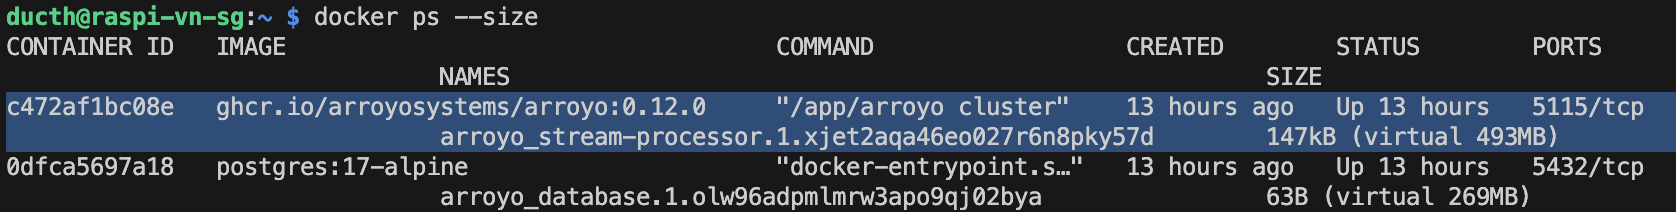
\includegraphics[width=\textwidth]{Images/docker_stack_deployment.png}
    \vspace{1em}
    \caption{Displaying deployment in Docker}
    \label{fig:docker_stack}
\end{figure}

In alignment with contemporary best practices in containerization and microservices architecture,
our deployment infrastructure leverages Docker Stack \cite{docker_stack} technology to orchestrate
and manage the operational components of our system, specifically focusing on two primary services:
the Arroyo server implementation and its associated PostgreSQL database instance. This containerized
approach not only ensures consistent deployment across different environments but also facilitates
sophisticated resource management and monitoring capabilities. Our performance analysis, as
illustrated in the accompanying system metrics visualization \ref{fig:docker_stack}, demonstrates
remarkably efficient resource utilization patterns, with both the Arroyo server and PostgreSQL
database maintaining notably conservative memory footprints that aggregate to approximately 800 MB
of total system memory consumption. This impressive resource efficiency validates our architectural
decisions and suggests substantial potential for scaling our implementation across various
deployment scenarios, from development environments to production systems, while maintaining optimal
performance characteristics and resource utilization patterns.

Our team source code for the \texttt{docker-compose.yaml} can be reviewed on our GitHub repository.

\subsection{Arroyo Console guide}
After successfully setting up and deploying Arroyo on our server infrastructure, we moved forward
with designing and implementing the monitoring pipeline that would help us achieve our project
objectives. Arroyo comes equipped with a user-friendly interface that makes the process of
developing and deploying data processing jobs surprisingly straightforward and intuitive. To begin
creating our monitoring solution, we simply navigated to the Arroyo Console, which serves as the
central hub for managing all pipeline-related operations. The interface presents a clean and
straightforward layout where users can find the \textbf{Create Pipeline} button prominently
displayed, marking the starting point for building new data processing workflows. This streamlined
approach to pipeline creation reflects Arroyo's overall design philosophy of making stream
processing more accessible while maintaining the powerful capabilities needed for complex data
analysis tasks. The simplicity of the interface proved to be a significant advantage for our team,
allowing us to focus more on the actual implementation of our monitoring logic rather than getting
caught up in complicated setup procedures or configuration details.

\begin{figure}[H]
    \centering
    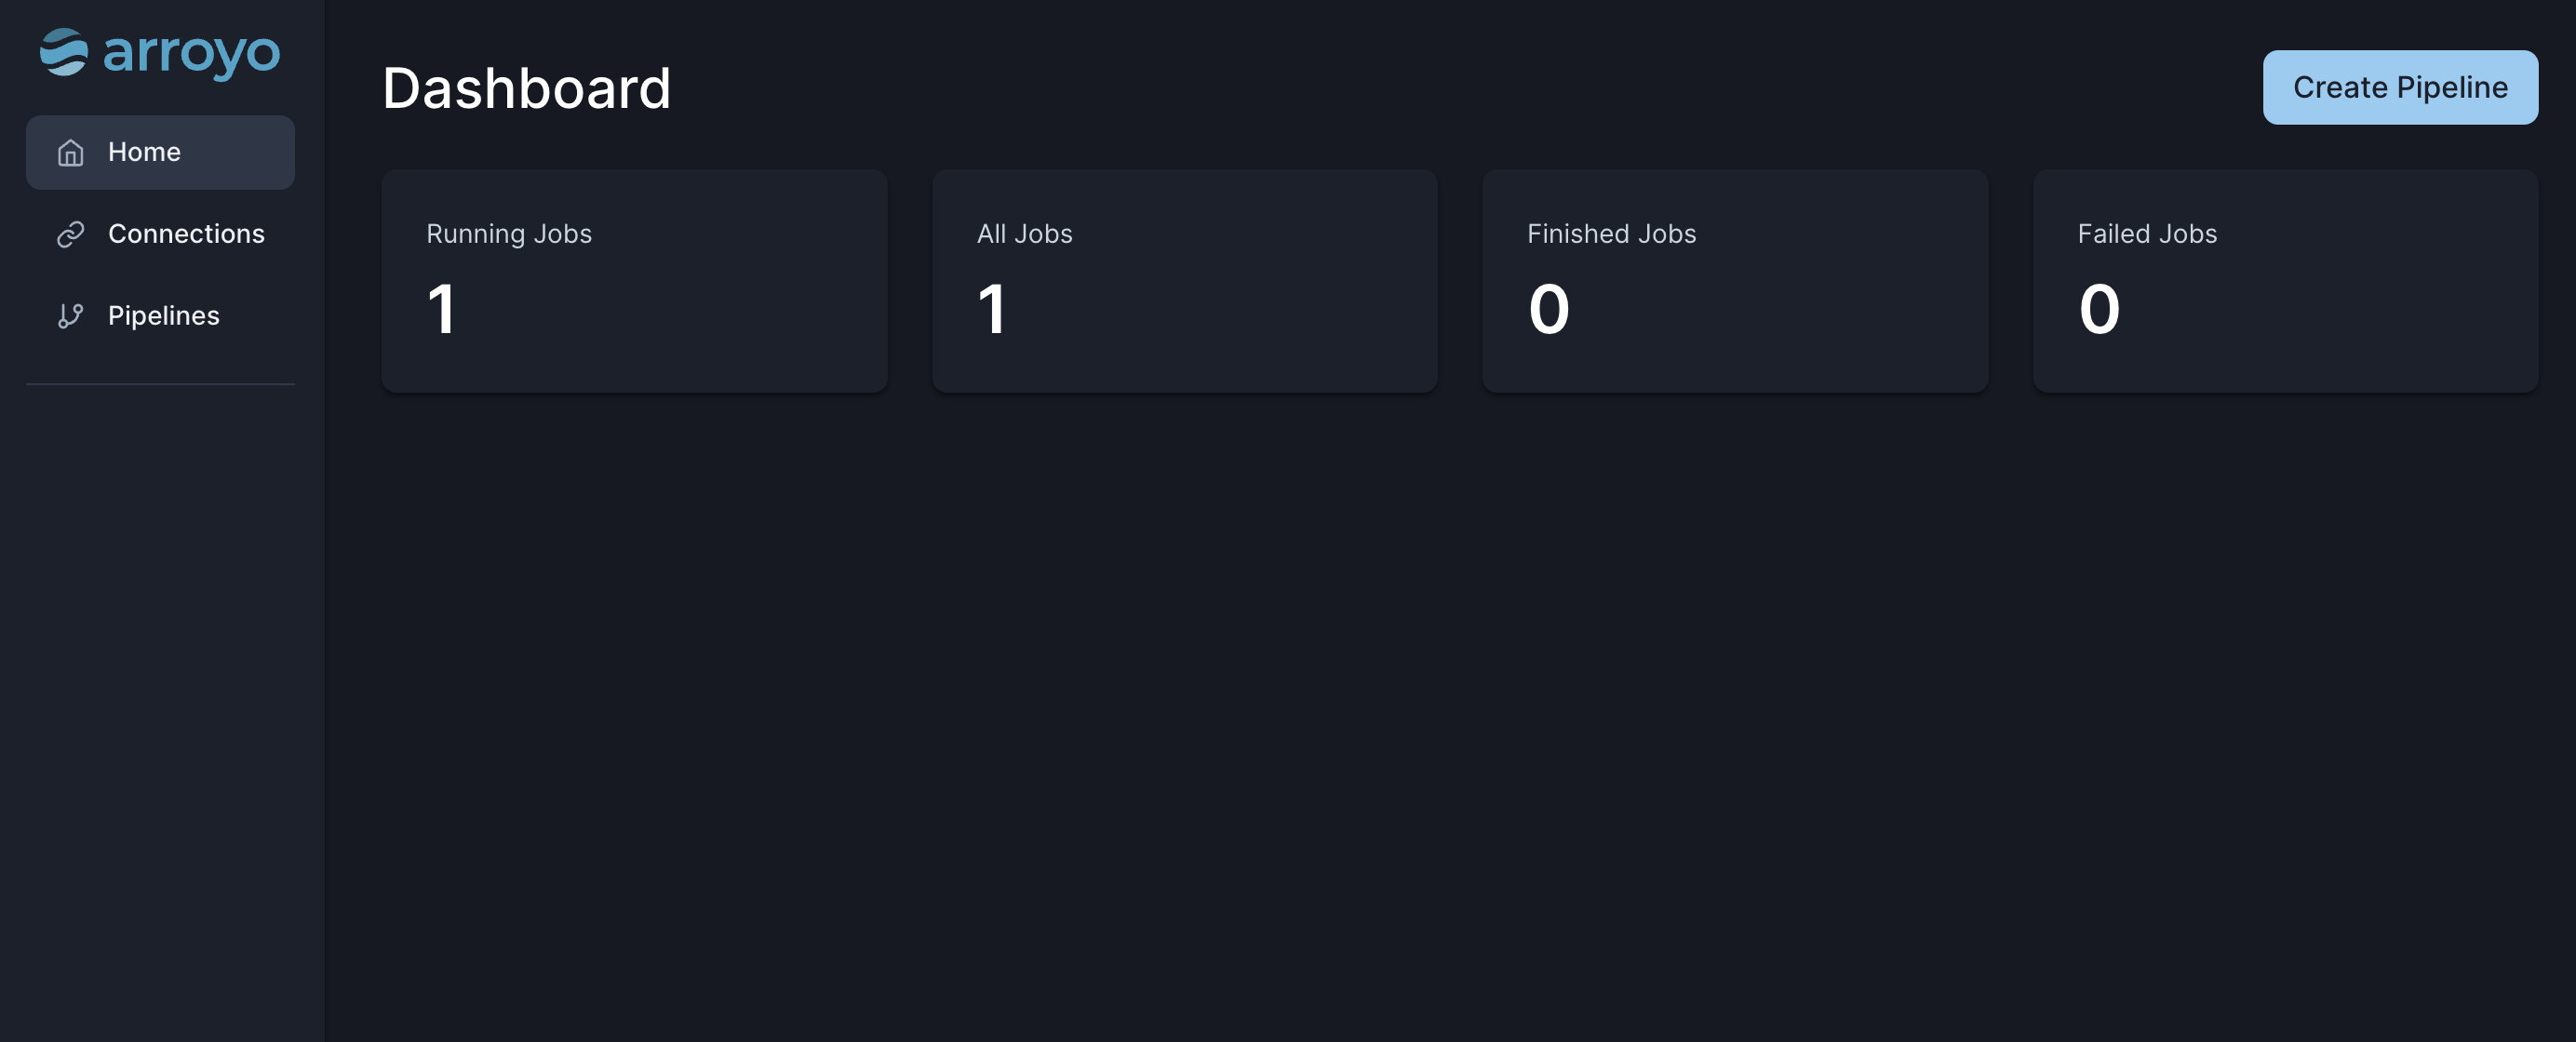
\includegraphics[width=\textwidth]{Images/arroyo_dashboard.png}
    \vspace{1em}
    \caption{Arroyo dashboard with our demo job running}
    \label{fig:arroyo_dashboard}
\end{figure}

Arroyo offers a straightforward and user-friendly Interactive Development Environment (IDE),
designed to simplify the process of working with data. Within this IDE, users can effortlessly write
SQL queries to read and manipulate data, enabling efficient calculations and transformations. The
\textbf{Preview} feature, accessible via the menubar, allows users to quickly preview the output of
their queries, providing immediate feedback and facilitating a more streamlined development cycle.
This rapid feedback loop helps users fine-tune their queries before proceeding to deployment. Once
the query meets the desired specifications, the \textbf{Launch} action can be used to deploy the
code for actual execution, making the transition from development to production both seamless and
efficient.

\begin{figure}[H]
    \centering
    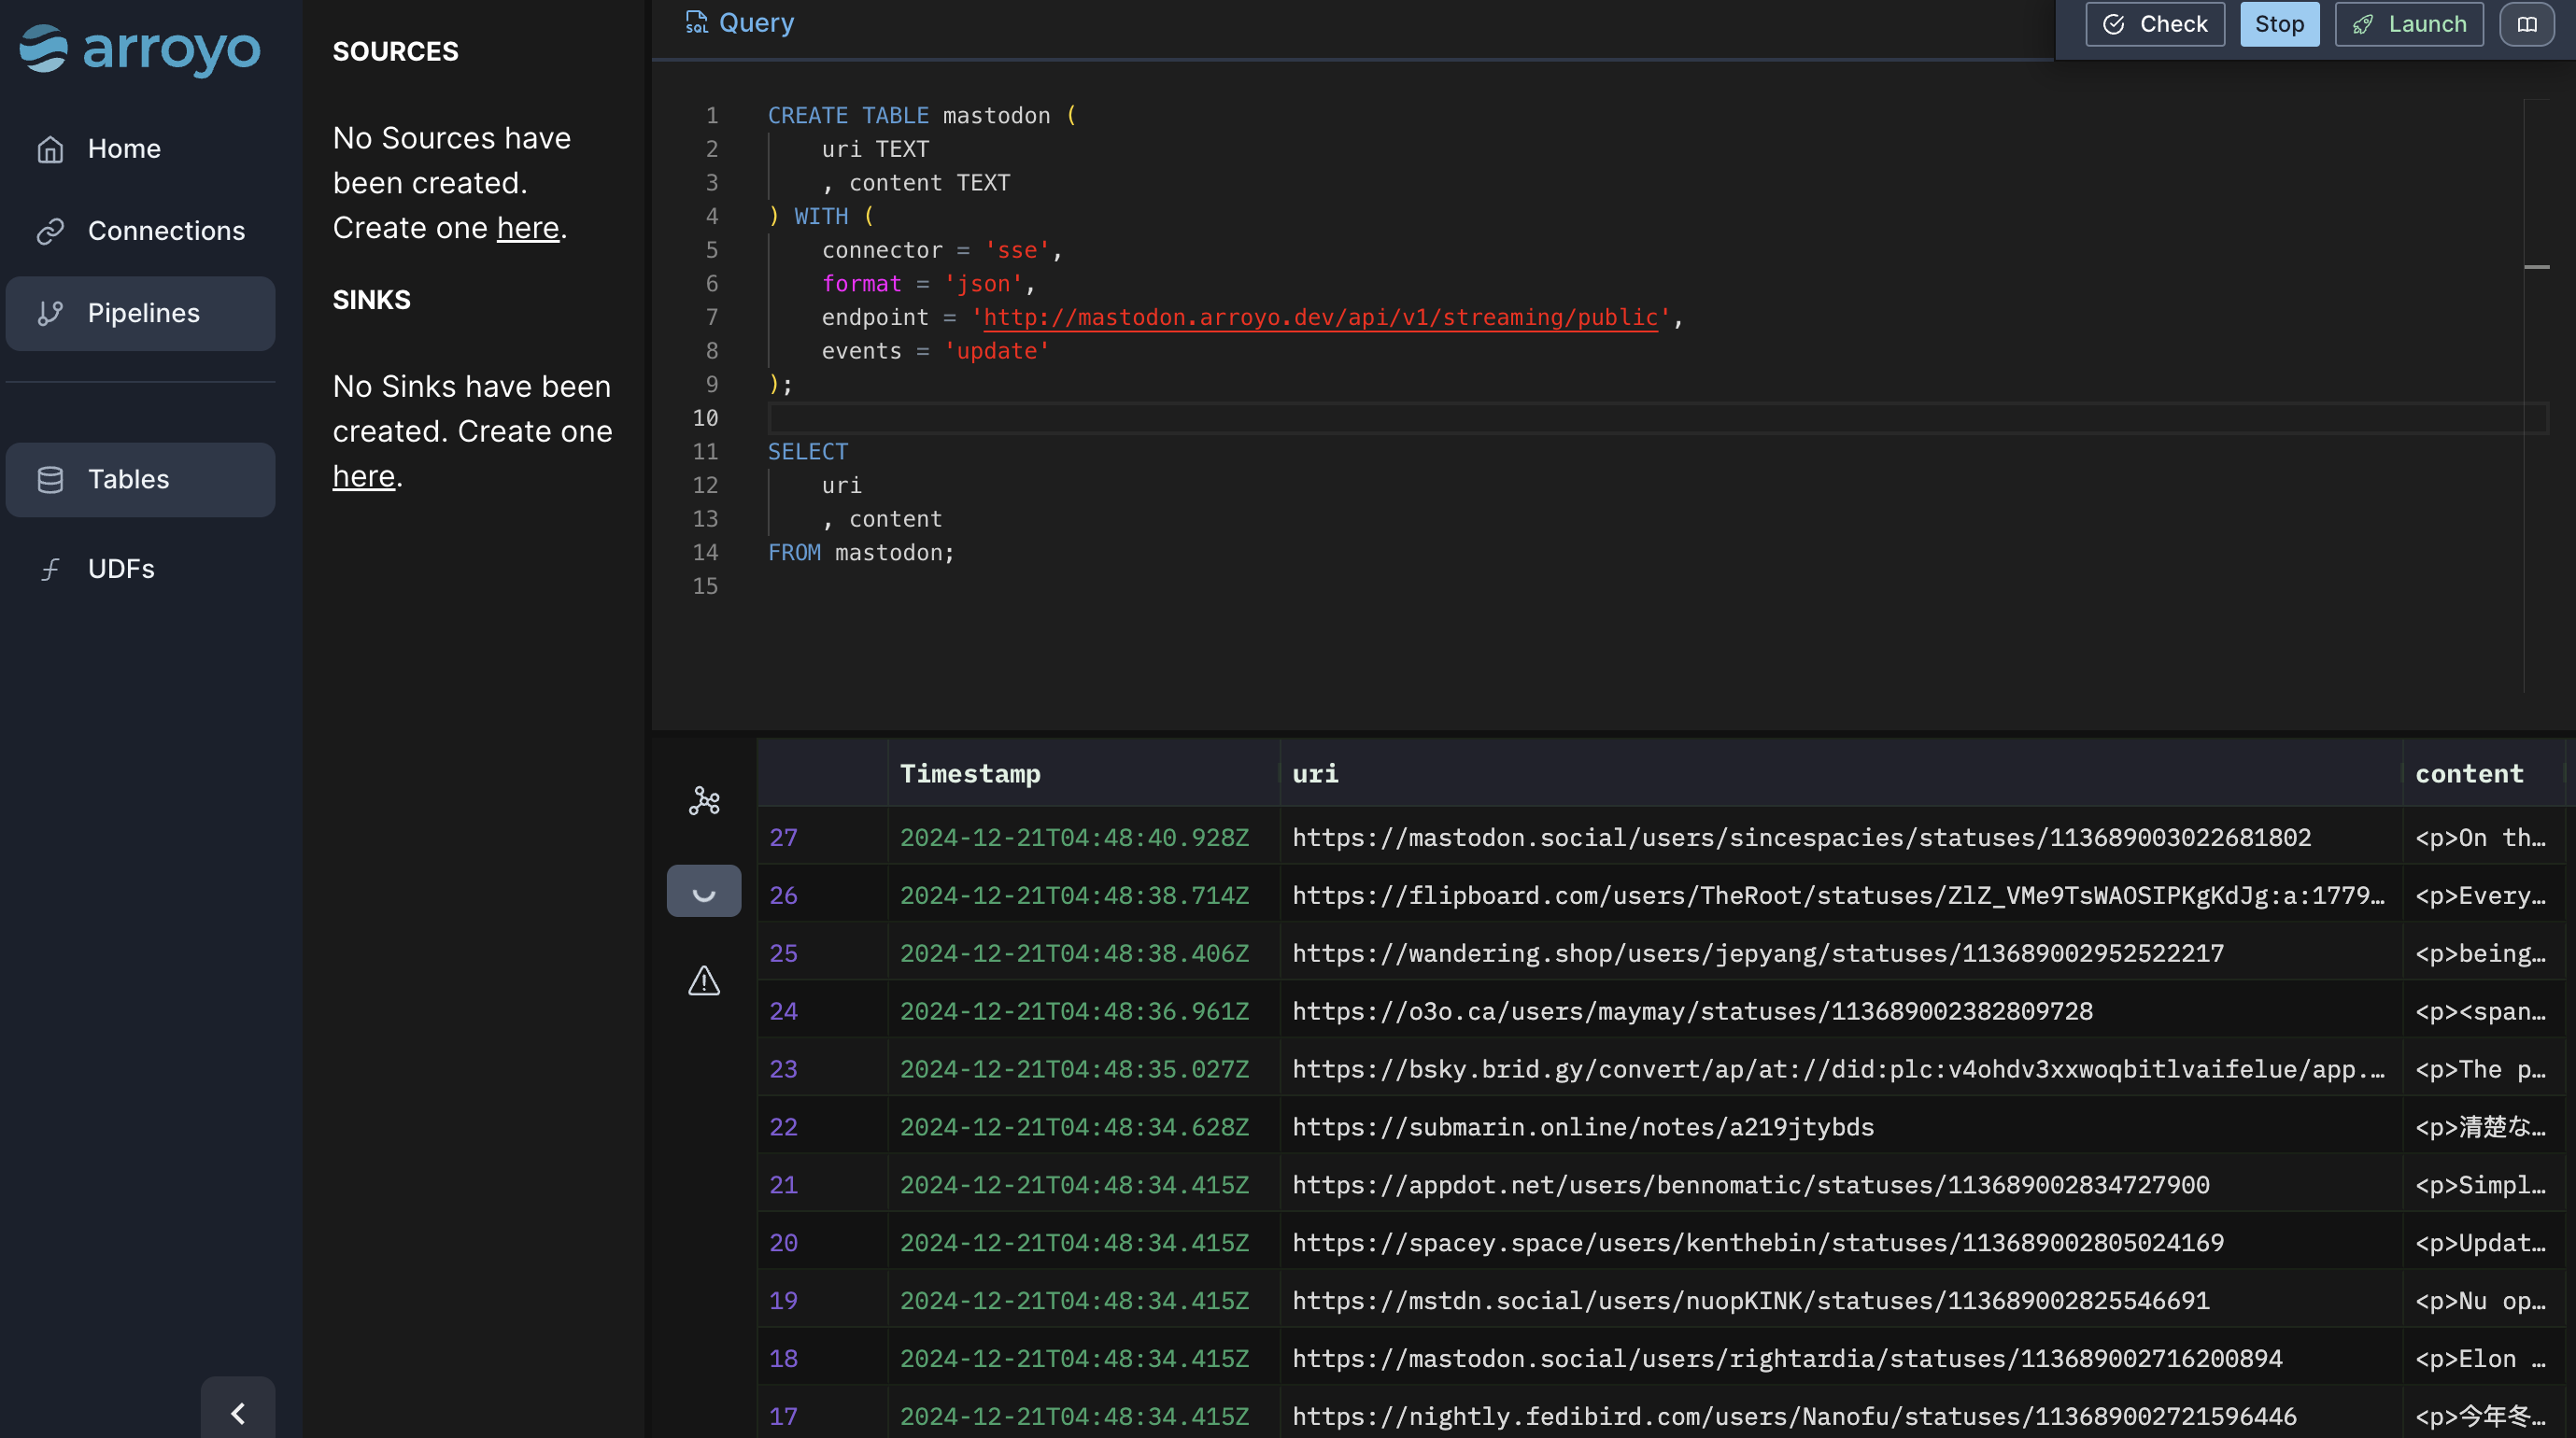
\includegraphics[width=\textwidth]{Images/arroyo_ide.png}
    \vspace{1em}
    \caption{Arroyo IDE}
    \label{fig:arroyo_ide}
\end{figure}

Arroyo also provides a highly intuitive dashboard that offers comprehensive monitoring capabilities
for running job details. This dashboard is equipped with a range of features designed to enhance
usability and insight: it visually represents the query tree or query plan of the task, enabling a
clear understanding of the job's structure; it allows users to tail the outputs of the job,
providing real-time visibility into its operation; and it offers detailed technical insights into
checkpoints, such as memory usage for each operator, the duration between operator lags, and other
performance metrics. These features collectively support a deeper understanding of the job's
behavior during deployment, making it easier for operators to quickly identify and address any
abnormalities or inefficiencies that may arise during execution.

\begin{figure}[H]
    \centering
    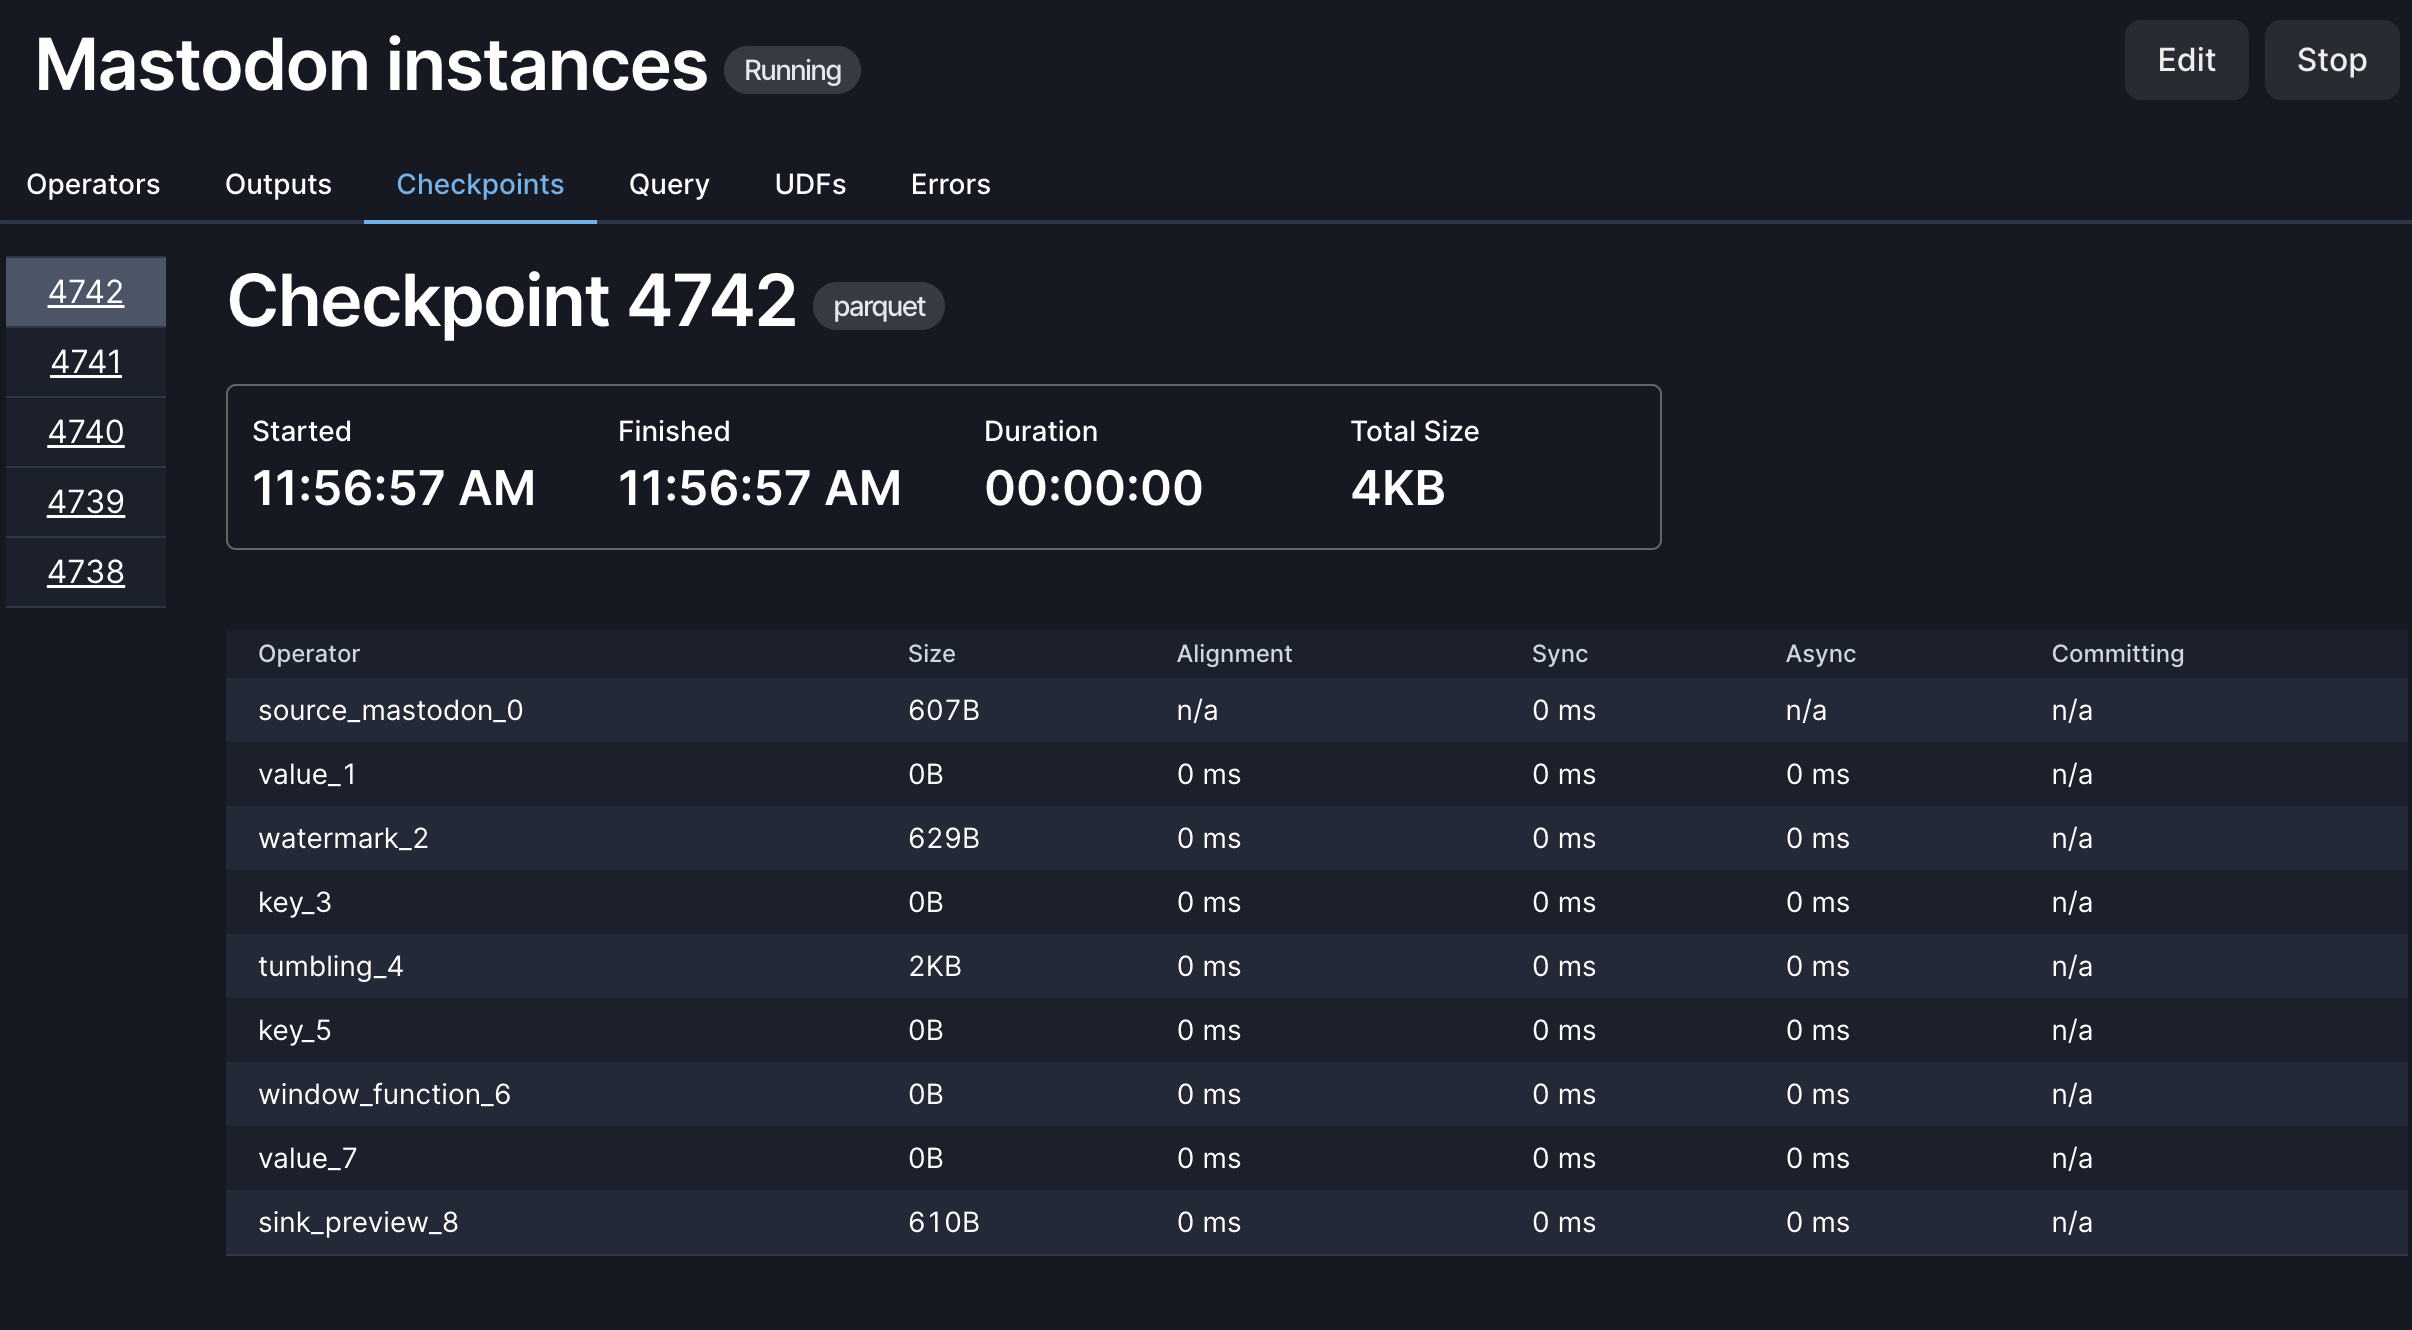
\includegraphics[width=\textwidth]{Images/arroyo_job_checkpoints.png}
    \vspace{1em}
    \caption{Details about a checkpoint of our demo job}
    \label{fig:arroyo_job_checkpoints}
\end{figure}

\subsection{Develop Instances Count Measurement}
We now describe in depth the code to accomplish the aforementioned objective.

\begin{lstlisting}[language=SQL]

CREATE TABLE mastodon (
    uri TEXT
) WITH (
    connector = 'sse',
    format = 'json',
    endpoint = 'http://mastodon.arroyo.dev/api/v1/streaming/public',
    events = 'update'
);

\end{lstlisting}

First, this snippet of code will create a \textbf{Source} for incoming data into the system. Here,
by using table as an abstraction, Arroyo simplifies the process of reading or writing to any other
system. Any type of messaging fabrics: Apache Kafka, MQTT or SSE can be represented in a relational
model. According to Mastodon documentation, incoming events are JSON-encoding, with a sample
structure similar to below. As you can see, the schema of the object has a high complexity.

\begin{lstlisting}[language=Python]
{
  "id": "108914327388663283",
  "created_at": "2022-08-30T23:05:46.839Z",
  "language": null,
  "uri": "https://letsalllovela.in/objects/e9cebb0c-7c75-414f-9608-20b5628e52d7",
  "content": "<span class=\"h-card\"><a class=\"u-url mention\" href=\"https://pl.nulled.red/users/disarray\" rel=\"nofollow noopener noreferrer\" target=\"_blank\">@<span>disarray</span></a></span> glad i was able to help",
  "account": {
    "id": "464472",
    "username": "freon",
    "acct": "freon@letsalllovela.in",
    "created_at": "2018-08-18T00:00:00.000Z",
    "emojis": [],
    "fields": [
      { "name": "pronouns", "value": "emacs/xemacs (or he/they)", "verified_at": null },
      { "name": "age", "value": "23.66667", "verified_at": null }
    ]
  },
  "media_attachments": [],
  "mentions": [
    { "id": "107946650784398271", "username": "disarray", "url": "https://pl.nulled.red/users/disarray", "acct": "disarray@pl.nulled.red" }
  ],
}
\end{lstlisting}

However, to achieve our result, we will focus primarily in the field \texttt{uri}. Because of this,
Arroyo helps us extract and parse this field into a separate column by setting the format to
\texttt{'json'}. That way, we can skip the step of actual parsing the JSON and get the property
(using Arroyo \texttt{json\_get} method).

\begin{lstlisting}[language=SQL]
WITH extract_domain AS (
    SELECT
        split_part(
            substr(uri, strpos(uri, '://') + 3),
            '/',
            1
        ) AS instance_domain
    FROM mastodon
)
\end{lstlisting}

Arroyo also supports the syntax of Common Table Expression (or CTE). This will support us with
enhancing code readability, by replacing nested \texttt{SELECT} statement with table representing
each step of the final transformation. For the first transformation, our team extracted the domain
name section from the URI, which should reside between a scheme (such as \texttt{https://}) and a
forward slash \texttt{/}. Arroyo SQL also supports many built-in string manipulation methods, like
\texttt{strpos} to find a position of a substring within a text, \texttt{substr} to extract a
substring between a beginning and ending position, and \texttt{split\_part} to split a string into
multiple substring based on a delimiter, and select a result of the splits.

\begin{lstlisting}[language=SQL]
, instance_domain_count AS (
    SELECT
        TUMBLE(interval '5 minutes') AS window
        , instance_domain
        , COUNT(*) AS cnt
    FROM extract_domain
    GROUP BY window, instance_domain
)
, instance_domain_sort AS (
    SELECT
        window
        , instance_domain
        , cnt
        , ROW_NUMBER() OVER (PARTITION BY window ORDER BY cnt DESC) AS order
    FROM instance_domain_count
)
SELECT
    window
    , instance_domain
    , cnt
FROM instance_domain_sort
WHERE order <= 5;
\end{lstlisting}

The next two steps is for our team to perform the complex aggregation on the incoming stream. To
achieve our object, we performed aggregation on data based on fixed-size, non-overlapping windows of
event incoming interval (which is also called \textbf{Tumbling Windows}). Then, we count for the
number of updates for each group of the instances. Finally, \texttt{ROW\_NUMBER()} is used to rank
the instance based on their event counts, partition per interval window. The final \texttt{SELECT}
then write out the result, but as we only interest in the top 5 mostly active instances, the
\texttt{WHERE} clause does the filtering step.

\begin{figure}[H]
    \centering
    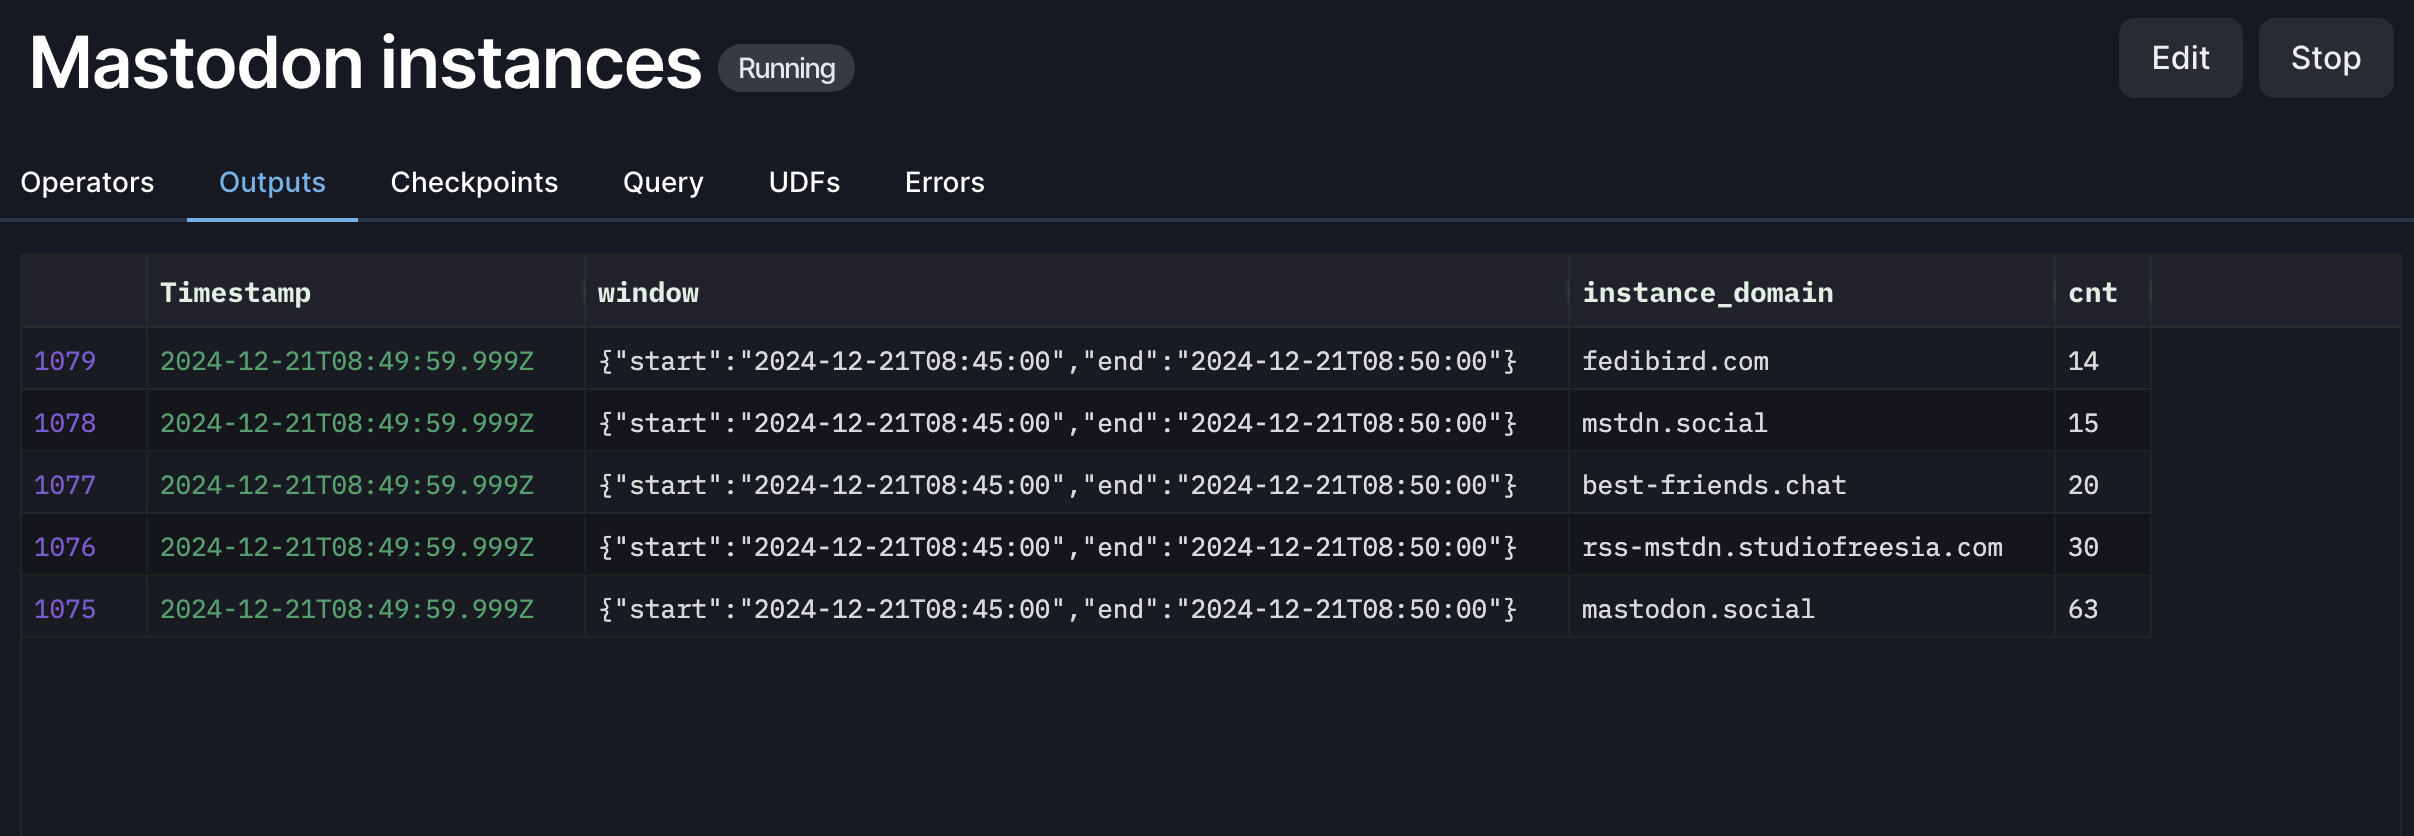
\includegraphics[width=\textwidth]{Images/mastodon_instance_count.png}
    \vspace{1em}
    \caption{Top 5 Mastodon instances within our sampling interval}
    \label{fig:mastodon_instance_count}
\end{figure}

The outcome is a table with a schema in figure \ref{fig:mastodon_instance_count}. Here, it includes
a window of processing interval, the domain name of the instance and its corresponding count. Most
of the time, \hyperref{https://mastodon.social/}{mastodon.social} will be the most active instance.
It was not a surprise when considering that this instance has a high popularity, and to most people
can be considered as the default server for Mastodon.
\section{Conclusion}
The deployment and operational insights gained from Arroyo highlight its exceptional suitability for
managing real-time social media interaction tracking tasks. Its core behavior, centered on efficient
stream processing and data analysis, underscores its capabilities as a modern tool optimized for
both scalability and precision. Arroyo demonstrates how distributed stream processing systems, such
as itself, can effectively bridge the gap between the volume and velocity of social media data
streams and the real-time analytics demanded by contemporary platforms.

Arroyo's design principles are apparent in its resource efficiency and ease of use. Written in Rust,
the framework offers significant performance benefits over traditional alternatives, as observed in
its low latency and minimal resource footprint, even when deployed on commodity hardware like the
Raspberry Pi. This outcome not only establishes Arroyo as a strong candidate for large-scale
applications but also showcases its adaptability to constrained environments, enabling broader
applications ranging from edge computing to traditional cloud environments.

The system's support for SQL-based streaming queries simplifies interaction and operational
complexity. By abstracting the intricacies of continuous data ingestion and processing, Arroyo
provides an accessible yet robust mechanism for monitoring and analyzing dynamic datasets, such as
the decentralized activities within Mastodon's federated network. This feature enhances its
usability for researchers, developers, and businesses aiming to derive actionable insights from
real-time data sources.

Moreover, its integration with widely used tools and protocols, such as Docker for deployment and
Server-Sent Events (SSE) APIs for real-time data fetching, ensures streamlined operational
workflows. Arroyo's built-in IDE and dashboard further simplify development and monitoring, offering
intuitive interfaces for query execution, job deployment, and resource tracking. These features
collectively foster an ecosystem that minimizes barriers to entry while maximizing productivity.

The demonstrated real-time tracking pipeline offers a clear testament to Arroyo's strength in
aggregating and analyzing unbounded data streams effectively. For instance, the ability to
dynamically identify the most active Mastodon instances within specific time windows provides not
only operational insights but also a foundation for exploring patterns within decentralized
networks. Such insights emphasize Arroyo's potential to contribute significantly to studies and
applications focused on evolving paradigms in social media and real-time analytics.

In summary, Arroyo's behavior reflects its potential as a versatile tool, efficiently addressing the
challenges associated with real-time data streams. Its implementation in this project affirms its
practical utility and paves the way for its application in diverse domains requiring similar
analytic capabilities.

\pagebreak
\section{Report links and details}
We also attached here, source codes and a presentation video based on this report.

\begin{enumerate}
    \item GitHub repo: \url{https://github.com/ducthuy-ng/bigdata-sem241}
    \item Presentation video: \url{https://www.youtube.com/watch?v=z8z_jYJGqDE}
\end{enumerate}

\pagebreak
\bibliographystyle{plainnat}
\bibliography{refs}

\nocite{*}

\end{document}